% Agile Orchestrators -- Innovation Challenge deck (v5).
% Content: agile-orchestrators-v4.pptx (the team's deck), plus the post-merge-docs skill.
% Look: the custom Rabobank design of ../agile-orchestrators/main.tex (override of the
% latex-presentation default preamble) and the team's Rabo reference visuals: navy/orange title
% band with gradient connector ring, italic blue titles, chevron phase bands, grey rounded
% columns with orange/green pills, thin blue line-art paths.
\documentclass[aspectratio=169,10pt]{beamer}
\usepackage[T1]{fontenc}
\usepackage[utf8]{inputenc}
\usepackage{lmodern}
\usepackage[scaled=0.92]{helvet}
\renewcommand{\familydefault}{\sfdefault}
\usepackage{amssymb}
\usepackage{tikz}
\usetikzlibrary{calc,positioning,arrows.meta,shapes.geometric,shapes.misc}

\graphicspath{{./images/}}

% ---------------------------------------------------------------- colours
\definecolor{raboNavy}{HTML}{000099}
\definecolor{raboBlue}{HTML}{0052FF}
\definecolor{raboLine}{HTML}{1C50D7}
\definecolor{raboOrange}{HTML}{FF6600}
\definecolor{raboGreen}{HTML}{03B463}
\definecolor{raboGrey}{HTML}{D9D9D9}
\definecolor{raboPanel}{HTML}{EDEDED}
\definecolor{raboLilac}{HTML}{E9E8F7}
\definecolor{raboPurple}{HTML}{7A2E8E}
\definecolor{raboInk}{HTML}{33334D}
\definecolor{raboMuted}{HTML}{8A8A99}
\definecolor{codeKey}{HTML}{FF8A3D}
\definecolor{codeText}{HTML}{E6E8FF}
\definecolor{codeMuted}{HTML}{9C9FE0}

% ---------------------------------------------------------------- beamer look
\setbeamertemplate{navigation symbols}{}
\setbeamersize{text margin left=0.8cm,text margin right=0.8cm}
\setbeamercolor{normal text}{fg=raboInk,bg=white}
\setbeamercolor{structure}{fg=raboBlue}
\setbeamercolor{alerted text}{fg=raboOrange}
\setbeamertemplate{itemize item}{\tikz[baseline=-0.55ex]\fill[raboOrange] (0,0) circle (1.5pt);}
\setbeamertemplate{itemize subitem}{\tikz[baseline=-0.55ex]\draw[raboBlue] (0,0) circle (1.2pt);}
\setlength{\leftmargini}{1.1em}
\hyphenpenalty=10000
\exhyphenpenalty=10000

\setbeamertemplate{frametitle}{%
  \vspace*{0.30cm}%
  {\color{raboBlue}\itshape\footnotesize\insertframesubtitle\par}%
  \vspace{0.5pt}%
  {\color{raboBlue}\itshape\fontsize{19}{21}\selectfont\insertframetitle\par}%
}

% Phase tracker (Prepare / Build / Close), drawn top right when \phaseno is 1, 2 or 3.
\def\phaseno{0}
\newcommand{\phasechev}[4]{% x, label, index, fill
  \ifnum#3=\phaseno
    \fill[#4] (#1,8.12) -- (#1+1.15,8.12) -- (#1+1.37,8.40) -- (#1+1.15,8.68) -- (#1,8.68)
      -- (#1+0.22,8.40) -- cycle;
    \node[text=white,font=\scriptsize\itshape\bfseries] at (#1+0.69,8.40) {#2};
  \else
    \fill[raboPanel] (#1,8.12) -- (#1+1.15,8.12) -- (#1+1.37,8.40) -- (#1+1.15,8.68) -- (#1,8.68)
      -- (#1+0.22,8.40) -- cycle;
    \node[text=raboMuted,font=\scriptsize\itshape] at (#1+0.69,8.40) {#2};
  \fi}

% Default background: page number bottom left, footer + logo bottom right.
\defbeamertemplate{background}{content}{%
  \begin{tikzpicture}
    \useasboundingbox (0,0) rectangle (16,9);
    \node[anchor=south east,inner sep=0] at (15.72,0.16)
      {
\includegraphics[height=0.70cm]{rabobank-logo}};
    \node[anchor=south east,text=raboBlue,font=\scriptsize\itshape,inner sep=0] at (15.02,0.24)
      {Agile Orchestrators \,\textperiodcentered\, Innovation Challenge};
    \node[anchor=south west,text=raboMuted,font=\tiny,inner sep=0] at (0.3,0.24)
      {\insertframenumber};
    \ifnum\phaseno>0
      \phasechev{11.05}{Prepare}{1}{raboOrange}
      \phasechev{12.36}{Build}{2}{raboGreen}
      \phasechev{13.67}{Close}{3}{raboNavy}
    \fi
  \end{tikzpicture}}
\setbeamertemplate{background}[content]

% Gradient ring used on the title and closing slides.
\newcommand{\connectorring}[3]{% centre x, centre y, radius
  \foreach \i in {0,...,59}{%
    \pgfmathsetmacro{\a}{215-\i*5.5}%
    \pgfmathtruncatemacro{\p}{100-\i*100/59}%
    \draw[line width=2.6pt,draw=raboOrange!\p!raboPurple]
      ($(#1,#2)+(\a:#3)$) arc[start angle=\a,end angle=\a-5.7,radius=#3];
  }%
  \draw[raboPurple!45,line width=0.5pt] ($(#1,#2)+(250:#3-0.28)$)
    arc[start angle=250,end angle=150,radius=#3-0.28];
}
\newcommand{\ringdot}[5]{% cx, cy, r, angle, label
  \pgfmathtruncatemacro{\q}{max(0,min(100,(215-#4)/3.3))}%
  \filldraw[fill=white,draw=raboOrange!\q!raboPurple,line width=1.3pt]
    ($(#1,#2)+(#4:#3)$) circle (0.17);
  \node[font=\tiny\itshape,text=raboInk,inner sep=1pt,anchor=#4+180] at ($(#1,#2)+(#4:#3+0.25)$) {#5};
}
% Title/closing layout: navy band, orange box, grey line, ring on the right.
\newcommand{\titlelayout}[4]{% band text, orange box text, grey line, ring script
  \begin{tikzpicture}
    \useasboundingbox (0,0) rectangle (16,9);
    \fill[raboOrange,rounded corners=1.5pt] (0.8,5.72) rectangle (1.02,5.94);
    \node[anchor=west,text=raboOrange,font=\small\bfseries,inner sep=0] at (1.15,5.83)
      {Innovation Challenge};
    \fill[raboNavy] (0,4.30) rectangle (9.9,5.45);
    \node[anchor=west,text=white,font=\fontsize{26}{28}\selectfont\itshape] at (0.8,4.86) {#1};
    \fill[raboOrange,rounded corners=5pt] (3.5,2.85) rectangle (9.9,4.10);
    \node[anchor=west,text=white,font=\normalsize\bfseries\itshape,text width=6.0cm,align=left]
      at (3.7,3.47) {#2};
    \node[anchor=north west,text=raboMuted,font=\scriptsize,text width=6.3cm,align=left]
      at (3.55,2.62) {#3};
    % thin line-art path leading into the ring
    \draw[raboLine,line width=0.7pt] (9.9,3.47) .. controls (10.6,3.47) and (10.4,4.2) .. (10.95,4.55);
    \fill[raboLine] (9.9,3.47) circle (2pt);
    \connectorring{12.55}{5.75}{2.05}
    \ringdot{12.55}{5.75}{2.05}{160}{Messaging}
    \ringdot{12.55}{5.75}{2.05}{112}{Email}
    \ringdot{12.55}{5.75}{2.05}{66}{Meeting notes}
    \ringdot{12.55}{5.75}{2.05}{20}{Documentation}
    \ringdot{12.55}{5.75}{2.05}{-26}{Project board}
    \ringdot{12.55}{5.75}{2.05}{-72}{Diagram tool}
    \node[align=center,font=\footnotesize,text=raboNavy] at (12.55,5.95)
      {\textbf{\large AI agent}\\[1pt] {\scriptsize AGILE ORCHESTRATORS}};
    \node[rotate=8,font=\small\itshape\bfseries,text=raboOrange] at (12.7,5.15) {#4};
    \node[anchor=south east,inner sep=0] at (15.6,0.35)
      {
\includegraphics[height=1.35cm]{rabobank-logo}};
  \end{tikzpicture}}

% ---------------------------------------------------------------- tikz styles
\tikzset{
  obox/.style={rounded corners=4pt,fill=raboOrange,text=white,align=center,
    font=\scriptsize,inner sep=3pt},
  gbox/.style={rounded corners=4pt,fill=raboGreen,text=white,align=center,
    font=\scriptsize,inner sep=3pt},
  nbox/.style={rounded corners=4pt,fill=raboNavy,text=white,align=center,
    font=\scriptsize,inner sep=3pt},
  wbox/.style={rounded corners=4pt,fill=white,draw=raboGrey,line width=0.8pt,text=raboInk,
    align=center,font=\scriptsize,inner sep=3pt},
  panel/.style={rounded corners=9pt,fill=raboPanel},
  line/.style={raboLine,line width=0.7pt},
  arr/.style={raboLine,line width=0.8pt,-{Stealth[length=2.2mm]}},
  htitle/.style={font=\small\itshape,text=raboBlue,anchor=north west,inner sep=0},
  body/.style={font=\scriptsize,text=raboInk,anchor=north west,inner sep=0,align=left},
  bubbleme/.style={fill=raboNavy,text=white,rounded corners=6pt,font=\small,inner sep=6pt,
    align=left},
  bubbleai/.style={fill=raboPanel,text=raboInk,rounded corners=6pt,font=\small,inner sep=6pt,
    align=left},
  callout/.style={fill=raboLilac,rounded corners=6pt,font=\scriptsize\itshape,text=raboNavy,
    inner sep=6pt,align=left,anchor=north west},
}
\newcommand{\sk}[1]{\texttt{#1}}

% One step of a phase: grey column, number on the line-art path, step, skill pill, context.
% x, width, number, step, skill, context, pill style
\newcommand{\stepcol}[7]{%
  \fill[panel] (#1,4.45) rectangle (#1+#2,1.55);
  \filldraw[fill=white,draw=raboLine,line width=0.9pt] (#1+#2/2,4.95) circle (0.27);
  \node[font=\scriptsize\bfseries\itshape,text=raboBlue] at (#1+#2/2,4.95) {#3};
  \node[font=\small\bfseries,text=raboNavy,align=center,text width=#2 cm-0.3cm]
    at (#1+#2/2,3.95) {#4};
  \node[#7,font=\scriptsize\ttfamily,minimum width=#2 cm-0.5cm,minimum height=0.55cm]
    at (#1+#2/2,3.2) {#5};
  \node[font=\tiny\itshape,text=raboMuted,anchor=north west,inner sep=0] at (#1+0.25,2.7)
    {Context it uses};
  \node[body,text width=#2 cm-0.5cm] at (#1+0.25,2.38) {#6};
}
% Thin line-art path behind the step numbers.
\newcommand{\steppath}[1]{% end x
  \draw[line] (0.1,4.95) -- (#1,4.95);
  \fill[raboLine] (0.1,4.95) circle (1.8pt);
  \draw[arr] (#1-0.4,4.95) -- (#1,4.95);
}

\begin{document}

% ================================================================ 1 title
{\setbeamertemplate{background}{\titlelayout{Agile Orchestrators}
   {AI agents for Agile\\ ways of working}
   {Adam Alansary \textperiodcentered\ Cedric Baron \textperiodcentered\ Jasper Krebbers
    \textperiodcentered\ Theun van Vliet \textperiodcentered\ Stefan Wachmann}
   {Scrum, orchestrated}}
 \begin{frame}[plain]\mbox{}\end{frame}}

% ================================================================ 2 challenge
\begin{frame}[t]{The challenge}{Situation \,\textperiodcentered\, complication \,\textperiodcentered\, question}
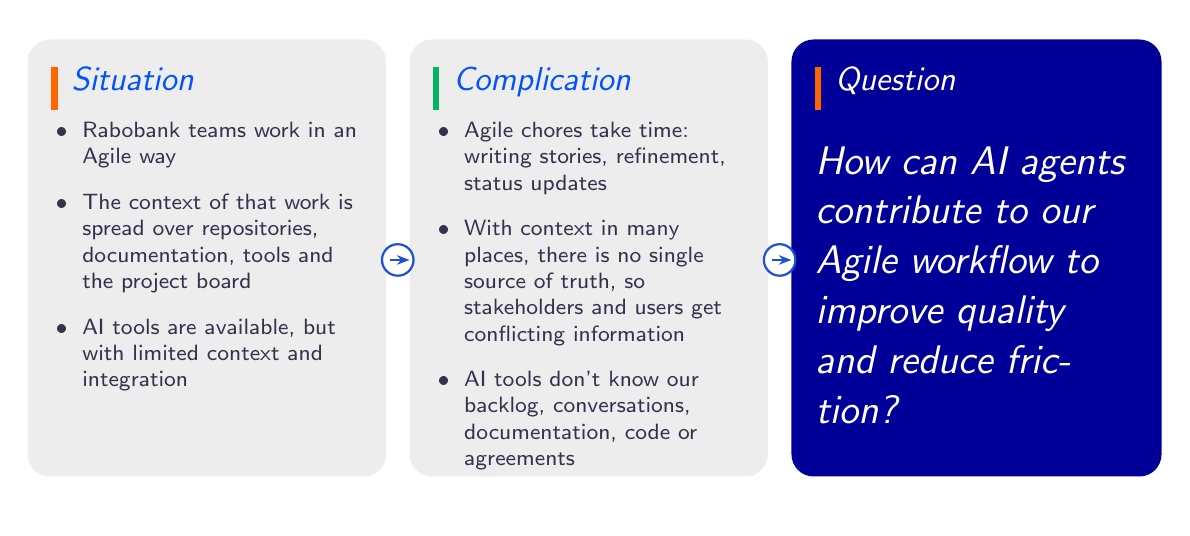
\begin{tikzpicture}
  \useasboundingbox (0,0) rectangle (14.4,6.1);
  \foreach \x/\c/\h/\items in {
    0/raboOrange/Situation/{
      \item Rabobank teams work in an Agile way
      \item The context of that work is spread over repositories, documentation, tools and
        the project board
      \item AI tools are available, but with limited context and integration},
    4.85/raboGreen/Complication/{
      \item Agile chores take time: writing stories, refinement, status updates
      \item With context in many places, there is no single source of truth, so stakeholders
        and users get conflicting information
      \item AI tools don't know our backlog, conversations, documentation, code or
        agreements}}{
    \fill[raboPanel,rounded corners=8pt] (\x,5.95) rectangle (\x+4.55,0.4);
    \fill[\c] (\x+0.3,5.6) rectangle (\x+0.38,5.05);
    \node[htitle,font=\large\itshape] at (\x+0.55,5.6) {\h};
    \node[body,text width=3.95cm,font=\footnotesize] at (\x+0.3,5.15)
      {\begin{itemize}\setlength{\itemsep}{5pt}\items\end{itemize}};
  }
  \fill[raboNavy,rounded corners=8pt] (9.7,5.95) rectangle (14.4,0.4);
  \fill[raboOrange] (10.0,5.6) rectangle (10.08,5.05);
  \node[htitle,font=\large\itshape,text=white] at (10.25,5.6) {Question};
  \node[anchor=north west,text=white,font=\fontsize{14}{18}\selectfont\itshape,
    text width=4.0cm,align=left,inner sep=0] at (10.0,4.6)
    {How can AI agents contribute to our Agile workflow to improve quality and reduce
     friction?};
  % line-art path tying the three panels together
  \foreach \x in {4.55,9.4}{
    \filldraw[fill=white,draw=raboLine,line width=0.8pt] (\x+0.15,3.15) circle (0.2);
    \draw[raboLine,line width=0.8pt,-{Stealth[length=1.6mm]}] (\x+0.05,3.15) -- (\x+0.3,3.15);
  }
\end{tikzpicture}
\end{frame}

% ================================================================ 3 test case
\begin{frame}[t]{Our test case: Tulip Bank}{A safe place to try it}
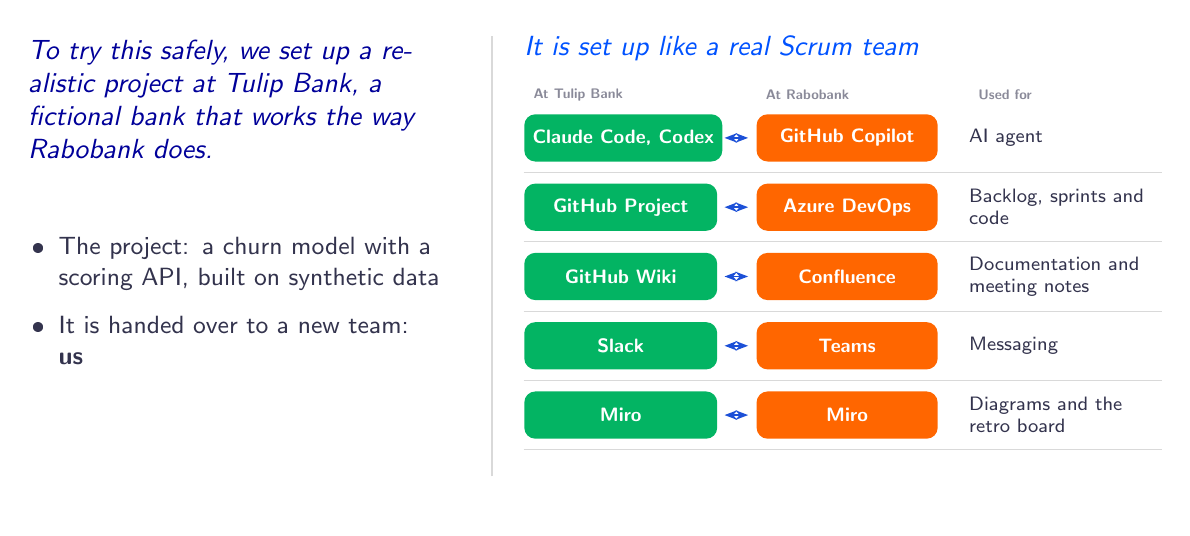
\begin{tikzpicture}
  \useasboundingbox (0,0) rectangle (14.4,6.1);
  \node[body,text width=5.3cm,font=\normalsize\itshape,text=raboNavy] at (0,5.95)
    {To try this safely, we set up a realistic project at Tulip Bank, a fictional bank that
     works the way Rabobank does.};
  \node[body,text width=5.3cm,font=\small] at (0,3.75) {%
    \begin{itemize}\setlength{\itemsep}{4.5pt}
      \item The project: a churn model with a scoring API, built on synthetic data
      \item It is handed over to a new team: \textbf{us}
    \end{itemize}};
  \draw[raboGrey,line width=0.6pt] (5.9,0.4) -- (5.9,6.0);
  \node[htitle,font=\normalsize\itshape] at (6.3,6.0) {It is set up like a real Scrum team};
  \foreach \t/\x in {At Tulip Bank/6.3,At Rabobank/9.25,Used for/11.95}{
    \node[anchor=west,font=\tiny\bfseries,text=raboMuted] at (\x,5.25) {\t};
  }
  \foreach \tb/\rb/\u [count=\i] in {
      {Claude Code, Codex}/GitHub Copilot/AI agent,
      GitHub Project/Azure DevOps/{Backlog, sprints and code},
      GitHub Wiki/Confluence/{Documentation and meeting notes},
      Slack/Teams/Messaging,
      Miro/Miro/{Diagrams and the retro board}}{
    \pgfmathsetmacro{\y}{4.7-(\i-1)*0.88}
    \node[gbox,anchor=west,minimum width=2.45cm,minimum height=0.6cm,font=\scriptsize\bfseries]
      at (6.3,\y) {\tb};
    \draw[line,{Stealth[length=1.6mm]}-{Stealth[length=1.6mm]}] (8.85,\y) -- (9.15,\y);
    \node[obox,anchor=west,minimum width=2.3cm,minimum height=0.6cm,font=\scriptsize\bfseries]
      at (9.25,\y) {\rb};
    \node[body,anchor=west,text width=2.4cm] at (11.95,\y) {\u};
    \draw[raboGrey,line width=0.4pt] (6.3,\y-0.44) -- (14.4,\y-0.44);
  }
\end{tikzpicture}
\end{frame}

% ================================================================ 4 context
\begin{frame}[t]{Getting started: giving the agent context}{Taking over the project}
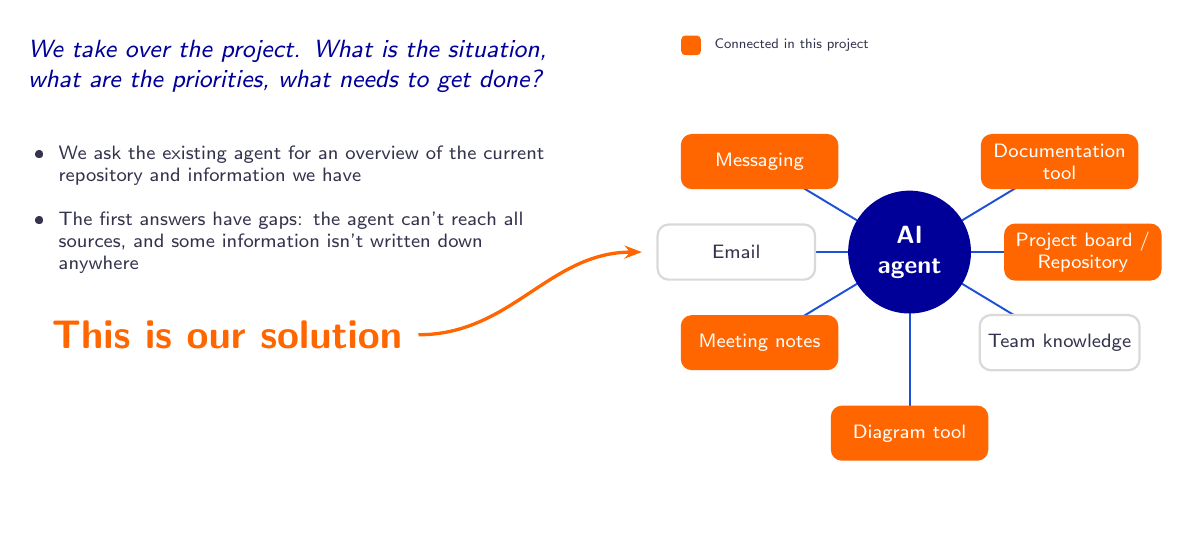
\begin{tikzpicture}
  \useasboundingbox (0,0) rectangle (14.4,6.1);
  \node[body,text width=6.6cm,font=\small\itshape,text=raboNavy] at (0,5.95)
    {We take over the project. What is the situation, what are the priorities, what needs to
     get done?};
  \node[body,text width=6.6cm] at (0,5.0) {%
    \begin{itemize}\setlength{\itemsep}{4pt}
      \item We ask the existing agent for an overview of the current repository and
        information we have
      \item The first answers have gaps: the agent can't reach all sources, and some
        information isn't written down anywhere
    \end{itemize}};
  % hub
  \coordinate (h) at (11.2,3.25);
  % lead-in from the bullets to the diagram
  \node[anchor=west,inner sep=0,font=\Large\bfseries\itshape,text=raboOrange] (sol)
    at (0.3,2.2) {This is our solution};
  \draw[arr,raboOrange,line width=1.2pt] ([xshift=0.2cm]sol.east)
    to[out=0,in=180] (7.8,3.25);
  \foreach \a/\t/\s in {150/Messaging/obox,30/{Documentation\\tool}/obox,
      180/Email/wbox,0/{Project board /\\Repository}/obox,210/{Meeting notes}/obox,
      -30/{Team knowledge}/wbox,-90/{Diagram tool}/obox}{
    \draw[line] (h) -- ($(h)+(\a:2.2 and 2.3)$);
    \node[\s,minimum width=2.0cm,minimum height=0.7cm] at ($(h)+(\a:2.2 and 2.3)$) {\t};
  }
  \fill[raboNavy] (h) circle (0.78);
  \node[text=white,font=\small\bfseries\itshape,align=center] at (h) {AI\\agent};
  \fill[raboOrange,rounded corners=1.5pt] (8.3,5.75) rectangle (8.55,6.0);
  \node[anchor=west,font=\tiny,text=raboInk] at (8.6,5.875) {Connected in this project};
\end{tikzpicture}
\end{frame}

% ================================================================ 5 skill
\begin{frame}[t]{What is a Skill?}{Recurring work, written down once}
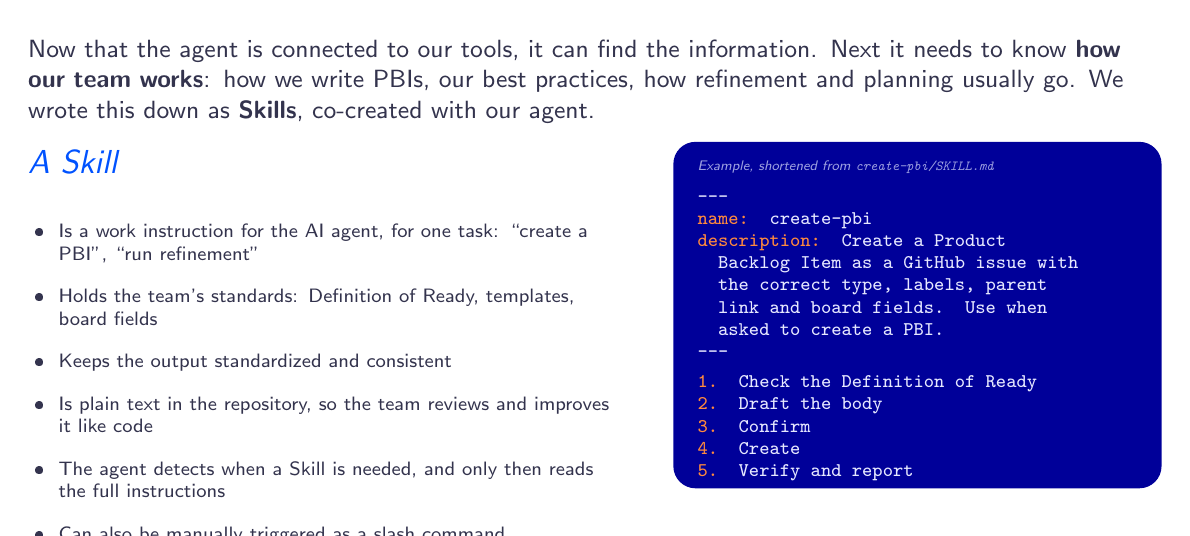
\begin{tikzpicture}
  \useasboundingbox (0,0) rectangle (14.4,6.1);
  \node[body,text width=14.2cm,font=\small] at (0,5.95)
    {Now that the agent is connected to our tools, it can find the information. Next it needs
     to know \textbf{how our team works}: how we write PBIs, our best practices, how refinement
     and planning usually go. We wrote this down as \textbf{Skills}, co-created with our
     agent.};
  \node[htitle,font=\large\itshape] at (0,4.55) {A Skill};
  \node[body,text width=7.4cm] at (0,4.0) {%
    \begin{itemize}\setlength{\itemsep}{3.5pt}
      \item Is a work instruction for the AI agent, for one task: ``create a PBI'', ``run
        refinement''
      \item Holds the team's standards: Definition of Ready, templates, board fields
      \item Keeps the output standardized and consistent
      \item Is plain text in the repository, so the team reviews and improves it like code
      \item The agent detects when a Skill is needed, and only then reads the full
        instructions
      \item Can also be manually triggered as a slash command
    \end{itemize}};
  \fill[raboNavy,rounded corners=8pt] (8.2,4.65) rectangle (14.4,0.25);
  \node[anchor=north west,inner sep=0,font=\tiny\itshape,text=codeMuted] at (8.5,4.42)
    {Example, shortened from \texttt{create-pbi/SKILL.md}};
  \node[anchor=north west,inner sep=0,font=\scriptsize\ttfamily,text=codeText,align=left]
    at (8.5,4.02) {%
    -{}-{}-\\
    {\color{codeKey}name:} create-pbi\\
    {\color{codeKey}description:} Create a Product\\
    \ \ Backlog Item as a GitHub issue with\\
    \ \ the correct type, labels, parent\\
    \ \ link and board fields. Use when\\
    \ \ asked to create a PBI.\\
    -{}-{}-\\[3pt]
    {\color{codeKey}1.} Check the Definition of Ready\\
    {\color{codeKey}2.} Draft the body\\
    {\color{codeKey}3.} Confirm\\
    {\color{codeKey}4.} Create\\
    {\color{codeKey}5.} Verify and report};
\end{tikzpicture}
\end{frame}

% ================================================================ 6 prepare
{\def\phaseno{1}
\begin{frame}[t]{Preparing the sprint}{The sprint lifecycle \,\textperiodcentered\, prepare}
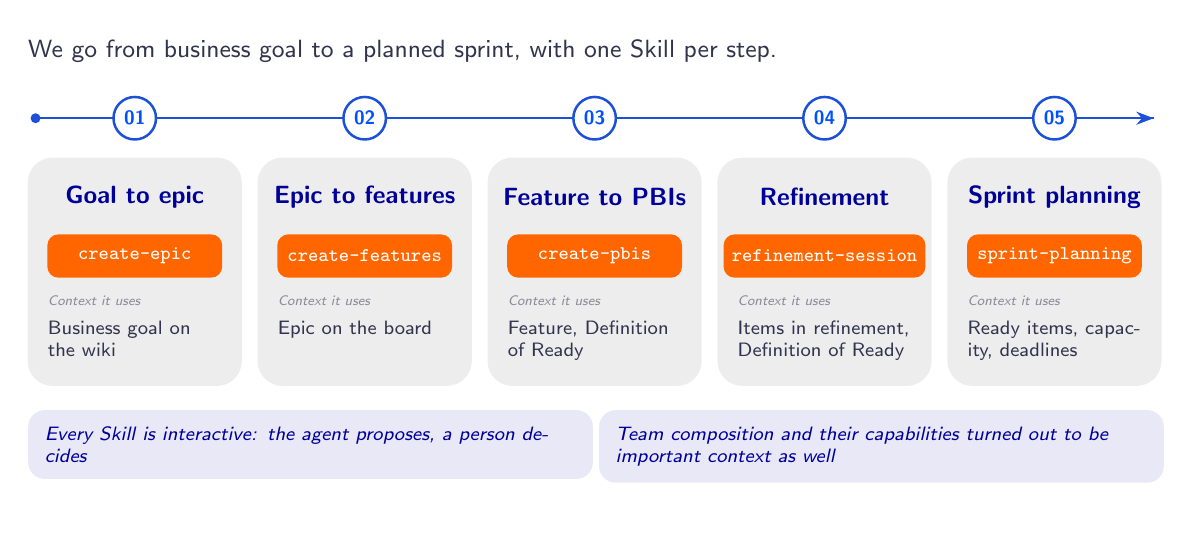
\begin{tikzpicture}
  \useasboundingbox (0,0) rectangle (14.4,6.1);
  \node[body,font=\small] at (0,5.95)
    {We go from business goal to a planned sprint, with one Skill per step.};
  \steppath{14.3}
  \stepcol{0}{2.72}{01}{Goal to epic}{create-epic}{Business goal on the wiki}{obox}
  \stepcol{2.92}{2.72}{02}{Epic to features}{create-features}{Epic on the board}{obox}
  \stepcol{5.84}{2.72}{03}{Feature to PBIs}{create-pbis}{Feature, Definition of Ready}{obox}
  \stepcol{8.76}{2.72}{04}{Refinement}{refinement-session}
    {Items in refinement, Definition of Ready}{obox}
  \stepcol{11.68}{2.72}{05}{Sprint planning}{sprint-planning}
    {Ready items, capacity, deadlines}{obox}
  \node[callout,text width=6.75cm] at (0,1.25)
    {Every Skill is interactive: the agent proposes, a person decides};
  \node[callout,text width=6.75cm] at (7.25,1.25)
    {Team composition and their capabilities turned out to be important context as well};
\end{tikzpicture}
\end{frame}}

% ================================================================ 8 build
{\def\phaseno{2}
\begin{frame}[t]{Doing the work}{The sprint lifecycle \,\textperiodcentered\, build}
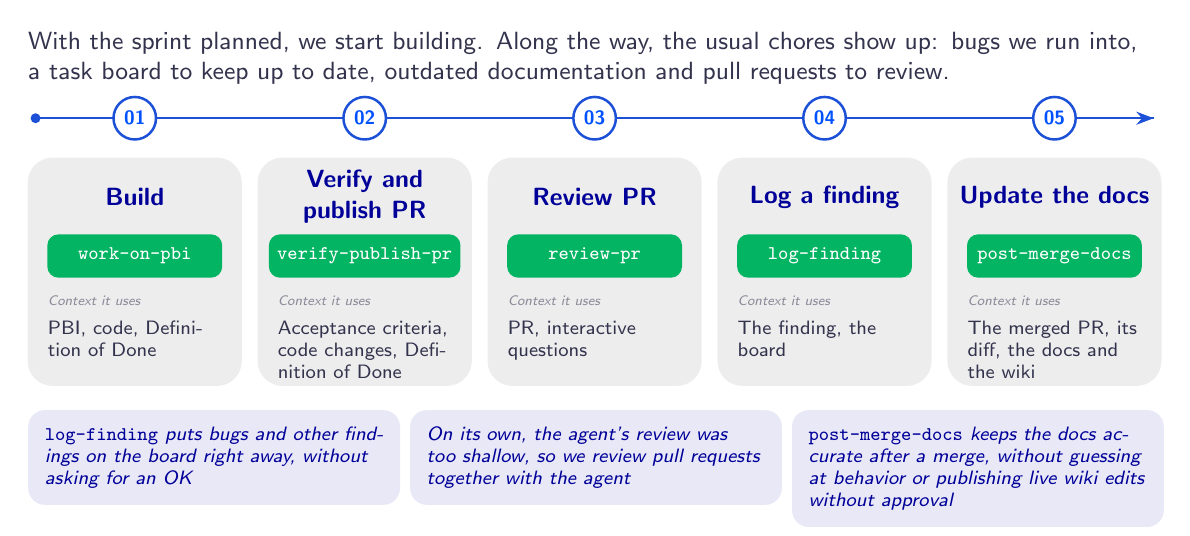
\begin{tikzpicture}
  \useasboundingbox (0,0) rectangle (14.4,6.1);
  \node[body,text width=14.3cm,font=\small] at (0,6.05)
    {With the sprint planned, we start building. Along the way, the usual chores show up: bugs
     we run into, a task board to keep up to date, outdated documentation and pull requests to
     review.};
  \steppath{14.3}
  \stepcol{0}{2.72}{01}{Build}{work-on-pbi}{PBI, code, Definition of Done}{gbox}
  \stepcol{2.92}{2.72}{02}{Verify and publish PR}{verify-publish-pr}
    {Acceptance criteria, code changes, Definition of Done}{gbox}
  \stepcol{5.84}{2.72}{03}{Review PR}{review-pr}{PR, interactive questions}{gbox}
  \stepcol{8.76}{2.72}{04}{Log a finding}{log-finding}{The finding, the board}{gbox}
  \stepcol{11.68}{2.72}{05}{Update the docs}{post-merge-docs}
    {The merged PR, its diff, the docs and the wiki}{gbox}
  \node[callout,text width=4.3cm] at (0,1.25)
    {\upshape\sk{log-finding} \itshape puts bugs and other findings on the board right away,
     without asking for an OK};
  \node[callout,text width=4.3cm] at (4.85,1.25)
    {On its own, the agent's review was too shallow, so we review pull requests together with
     the agent};
  \node[callout,text width=4.3cm] at (9.7,1.25)
    {\upshape\sk{post-merge-docs} \itshape keeps the docs accurate after a merge, without
     guessing at behavior or publishing live wiki edits without approval};
\end{tikzpicture}
\end{frame}}

% ================================================================ 9 close
{\def\phaseno{3}
\begin{frame}[t]{Closing the sprint}{The sprint lifecycle \,\textperiodcentered\, close}
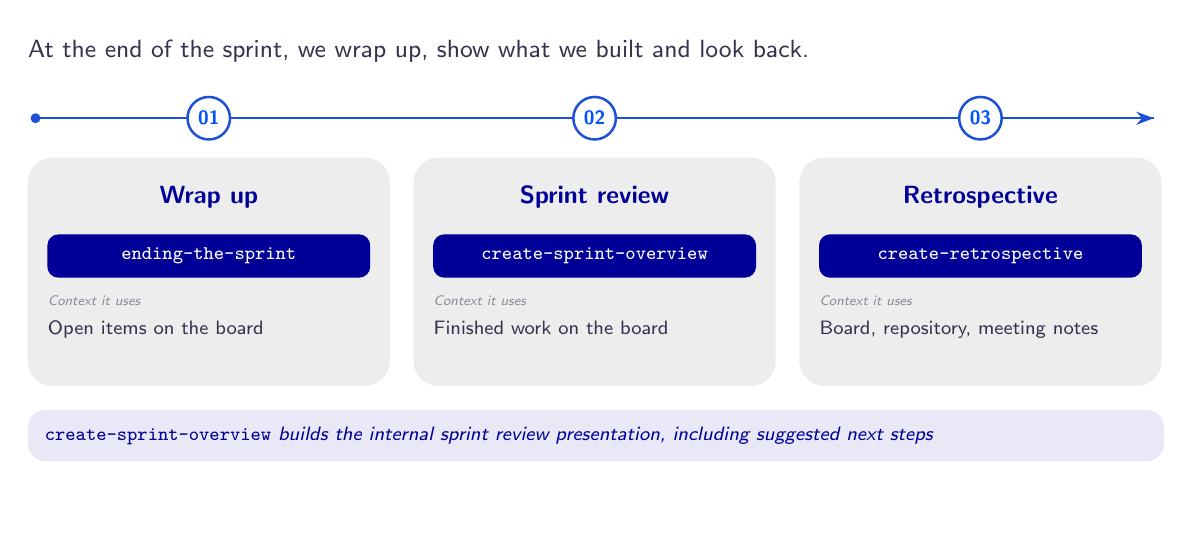
\begin{tikzpicture}
  \useasboundingbox (0,0) rectangle (14.4,6.1);
  \node[body,font=\small] at (0,5.95)
    {At the end of the sprint, we wrap up, show what we built and look back.};
  \steppath{14.3}
  \stepcol{0}{4.6}{01}{Wrap up}{ending-the-sprint}{Open items on the board}{nbox}
  \stepcol{4.9}{4.6}{02}{Sprint review}{create-sprint-overview}{Finished work on the board}{nbox}
  \stepcol{9.8}{4.6}{03}{Retrospective}{create-retrospective}
    {Board, repository, meeting notes}{nbox}
  \node[callout,text width=14.0cm] at (0,1.25)
    {\upshape\sk{create-sprint-overview} \itshape builds the internal sprint review
     presentation, including suggested next steps};
\end{tikzpicture}
\end{frame}}

% ================================================================ 10 retro example
{\def\phaseno{3}
\begin{frame}[t]{Example: retrospective}{The sprint lifecycle \,\textperiodcentered\, close}
\begin{tikzpicture}
  \useasboundingbox (0,0) rectangle (14.4,6.1);
  \node[anchor=north west,inner sep=0] (img) at (0,5.95)
    {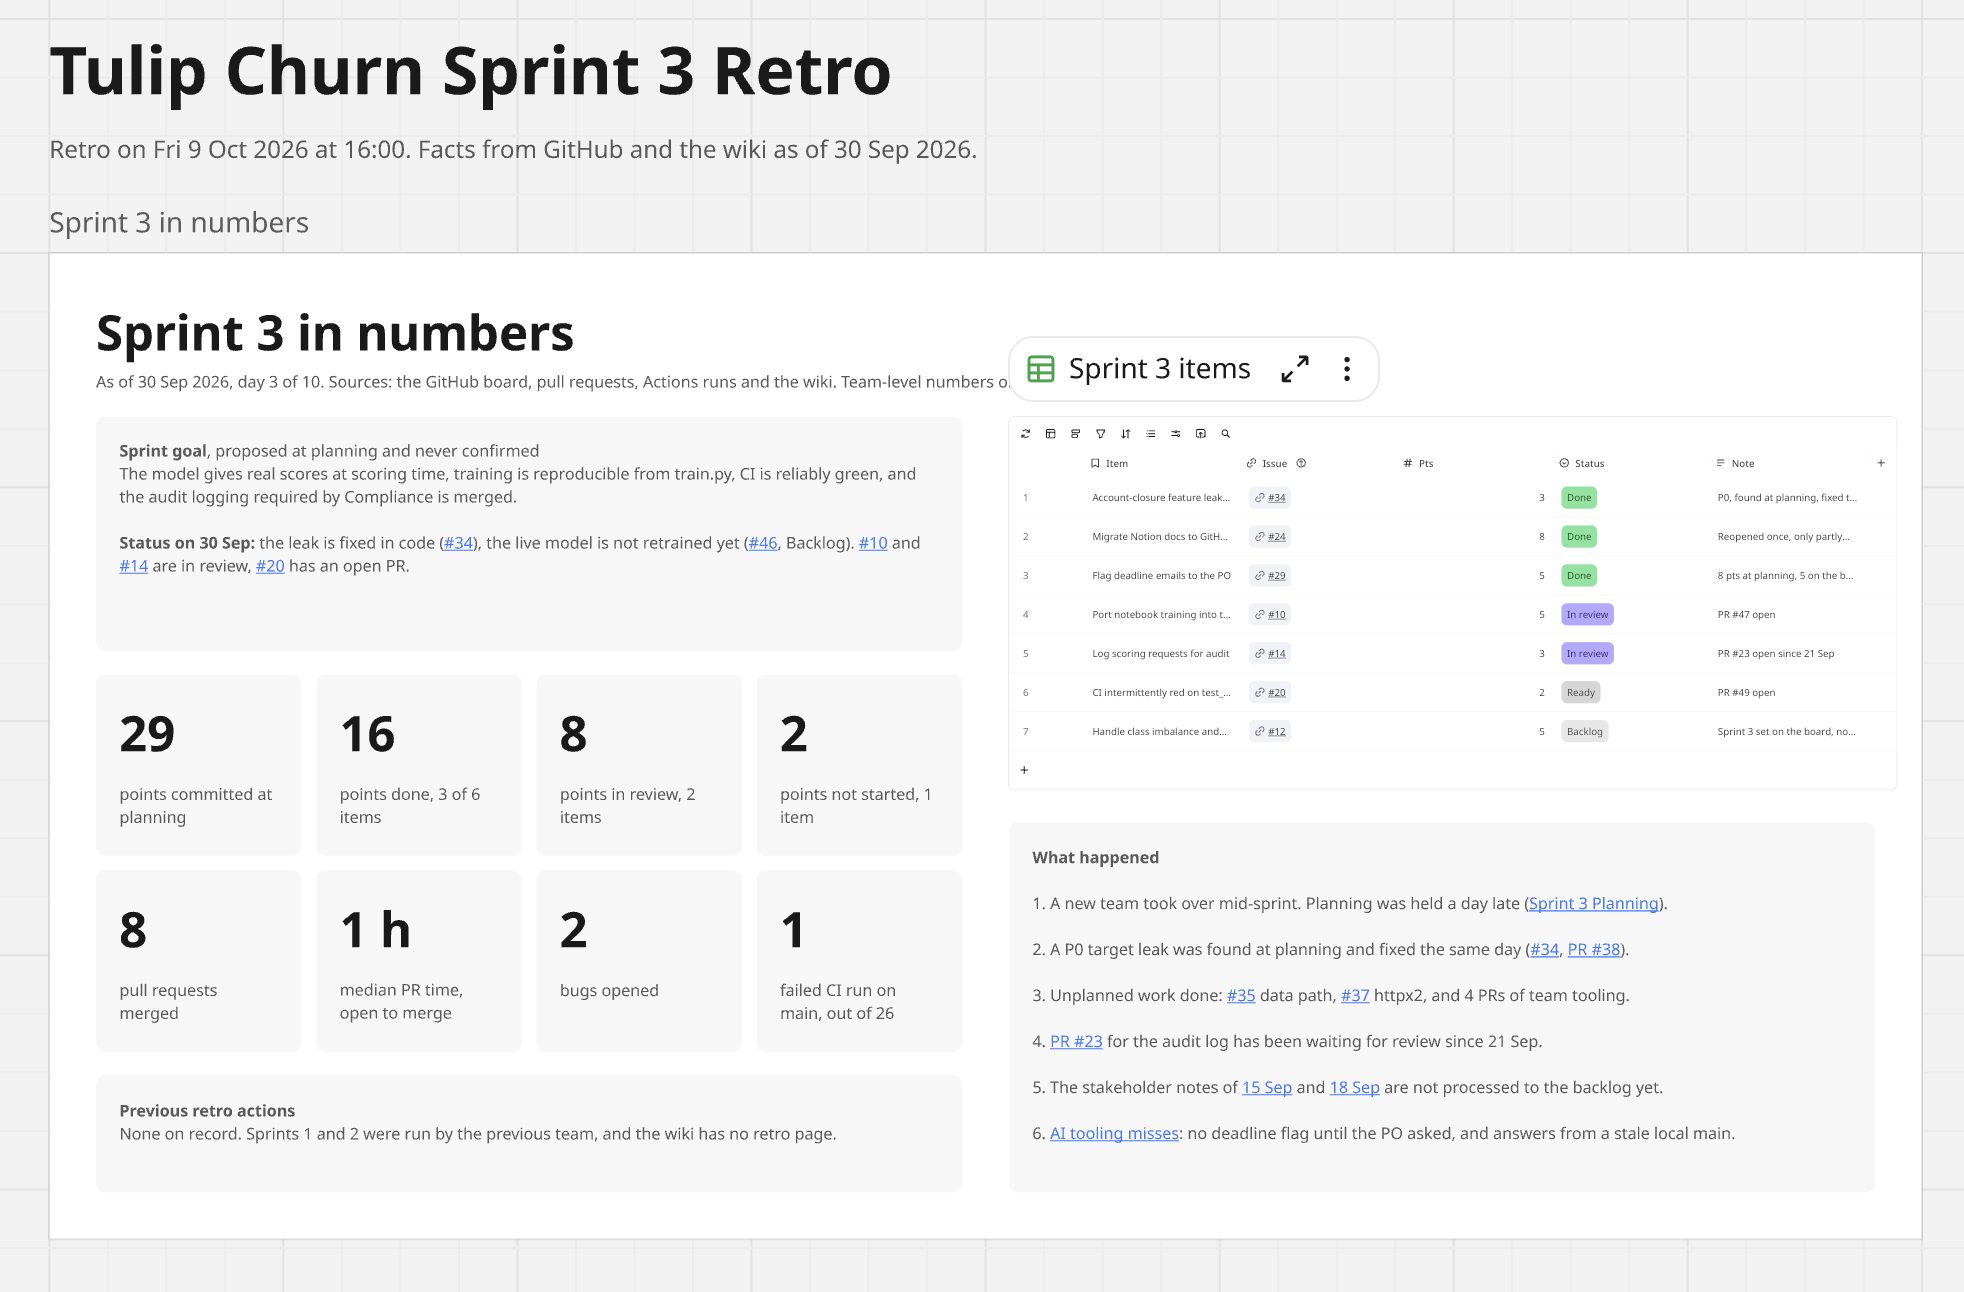
\includegraphics[width=8.0cm]{retro-miro-board}};
  \draw[raboGrey,line width=0.6pt,rounded corners=2pt] (img.south west) rectangle (img.north east);
  \node[anchor=east,font=\tiny\bfseries,text=raboMuted] at (14.4,5.9) {Prompt};
  \node[bubbleme,anchor=north east] at (14.4,5.7) {Start the retro.};
  \node[anchor=west,font=\tiny\bfseries,text=raboMuted] at (8.6,4.6) {Agent};
  \node[bubbleai,anchor=north west,text width=5.4cm] at (8.6,4.4)
    {The retro board is ready in Miro. I've added talking points from the sprint, the
     sprint's metrics and links to the project board for quick access.};
  \draw[line] (8.6,1.95) -- (8.6,0.75);
  \node[anchor=north west,text width=5.5cm,font=\normalsize\itshape,text=raboBlue,inner sep=0,
    align=left] at (8.85,1.95)
    {The agent does the preparation, so the team can spend the retro on the conversation};
\end{tikzpicture}
\end{frame}}

% ================================================================ 11 learned / next
\begin{frame}[t]{What we learned and what's next}{Lessons that carry over}
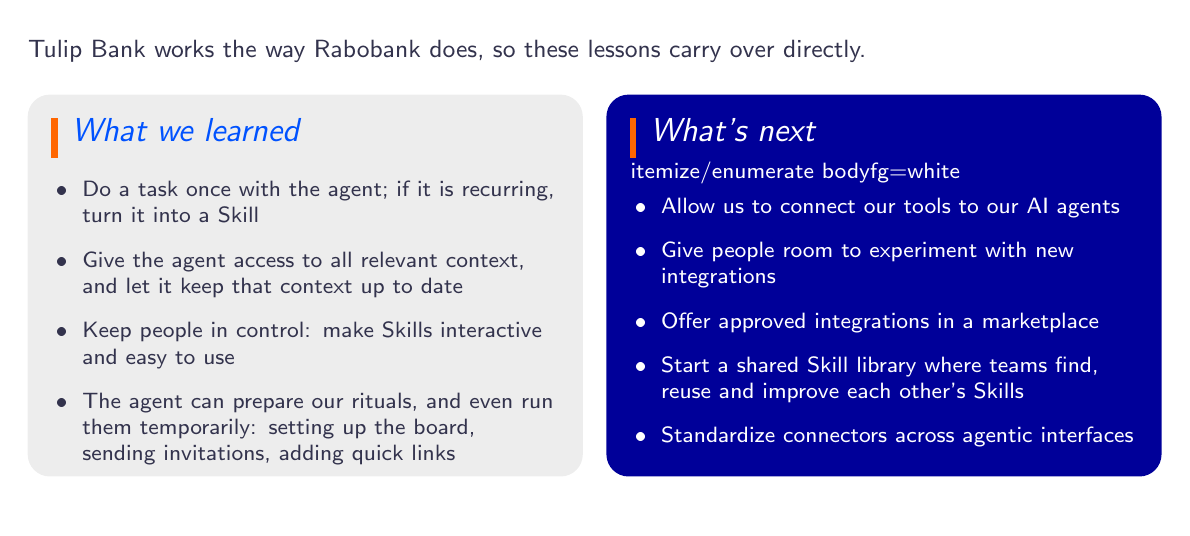
\begin{tikzpicture}
  \useasboundingbox (0,0) rectangle (14.4,6.1);
  \node[body,font=\small] at (0,5.95)
    {Tulip Bank works the way Rabobank does, so these lessons carry over directly.};
  \fill[raboPanel,rounded corners=8pt] (0,5.25) rectangle (7.05,0.4);
  \fill[raboOrange] (0.3,4.95) rectangle (0.38,4.45);
  \node[htitle,font=\large\itshape] at (0.55,4.95) {What we learned};
  \node[body,text width=6.4cm,font=\footnotesize] at (0.3,4.4) {%
    \begin{itemize}\setlength{\itemsep}{4.5pt}
      \item Do a task once with the agent; if it is recurring, turn it into a Skill
      \item Give the agent access to all relevant context, and let it keep that context up to
        date
      \item Keep people in control: make Skills interactive and easy to use
      \item The agent can prepare our rituals, and even run them temporarily: setting up the
        board, sending invitations, adding quick links
    \end{itemize}};
  \fill[raboNavy,rounded corners=8pt] (7.35,5.25) rectangle (14.4,0.4);
  \fill[raboOrange] (7.65,4.95) rectangle (7.73,4.45);
  \node[htitle,font=\large\itshape,text=white] at (7.9,4.95) {What's next};
  \node[body,text width=6.4cm,font=\footnotesize,text=white] at (7.65,4.4) {%
    \setbeamercolor{itemize/enumerate body}{fg=white}\color{white}%
    \begin{itemize}\setlength{\itemsep}{4.5pt}
      \item Allow us to connect our tools to our AI agents
      \item Give people room to experiment with new integrations
      \item Offer approved integrations in a marketplace
      \item Start a shared Skill library where teams find, reuse and improve each other's
        Skills
      \item Standardize connectors across agentic interfaces
    \end{itemize}};
\end{tikzpicture}
\end{frame}

% ================================================================ 12 appendix slopguard
\begin{frame}[t]{Appendix: slopguard}{Keeping agent-written code clean}
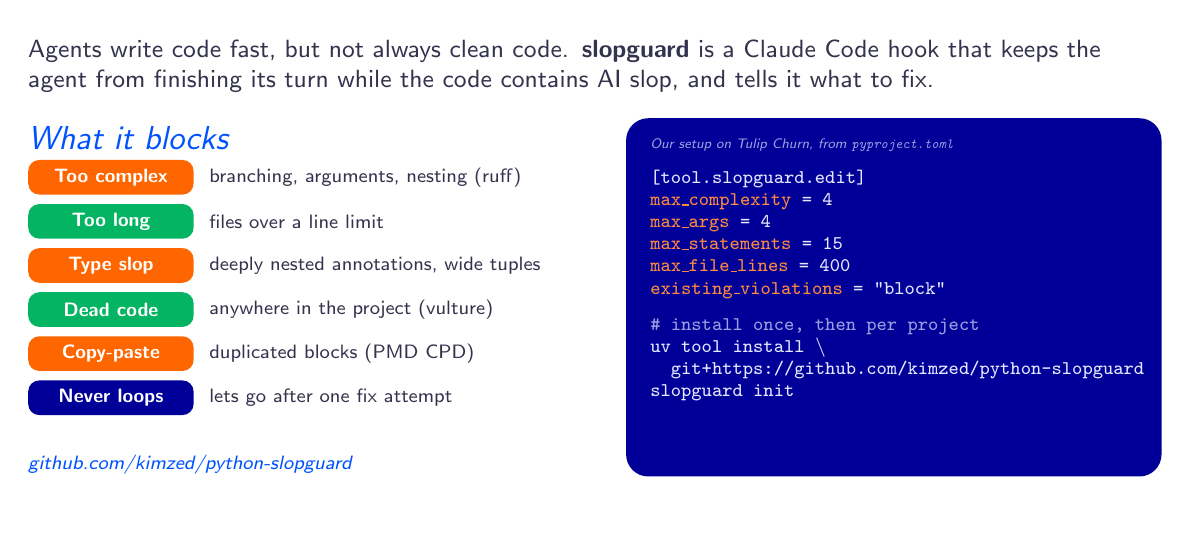
\begin{tikzpicture}
  \useasboundingbox (0,0) rectangle (14.4,6.1);
  \node[body,text width=14.2cm,font=\small] at (0,5.95)
    {Agents write code fast, but not always clean code. \textbf{slopguard} is a Claude Code
     hook that keeps the agent from finishing its turn while the code contains AI slop, and
     tells it what to fix.};
  \node[htitle,font=\large\itshape] at (0,4.85) {What it blocks};
  \foreach \t/\d/\c [count=\i] in {
      Too complex/{branching, arguments, nesting (ruff)}/obox,
      Too long/{files over a line limit}/gbox,
      Type slop/{deeply nested annotations, wide tuples}/obox,
      Dead code/{anywhere in the project (vulture)}/gbox,
      Copy-paste/{duplicated blocks (PMD CPD)}/obox,
      Never loops/{lets go after one fix attempt}/nbox}{
    \pgfmathsetmacro{\y}{4.2-(\i-1)*0.56}
    \node[\c,anchor=west,minimum width=2.1cm,minimum height=0.44cm,font=\scriptsize\bfseries]
      at (0,\y) {\t};
    \node[body,anchor=west] at (2.3,\y) {\d};
  }
  \node[anchor=west,font=\scriptsize\itshape,text=raboBlue,inner sep=0] at (0,0.55)
    {github.com/kimzed/python-slopguard};
  \fill[raboNavy,rounded corners=8pt] (7.6,4.95) rectangle (14.4,0.4);
  \node[anchor=north west,inner sep=0,font=\tiny\itshape,text=codeMuted] at (7.9,4.7)
    {Our setup on Tulip Churn, from \texttt{pyproject.toml}};
  \node[anchor=north west,inner sep=0,font=\scriptsize\ttfamily,text=codeText,align=left]
    at (7.9,4.3) {%
    [tool.slopguard.edit]\\
    {\color{codeKey}max\_complexity} = 4\\
    {\color{codeKey}max\_args} = 4\\
    {\color{codeKey}max\_statements} = 15\\
    {\color{codeKey}max\_file\_lines} = 400\\
    {\color{codeKey}existing\_violations} = "block"\\[5pt]
    {\color{codeMuted}\# install once, then per project}\\
    uv tool install \textbackslash\\
    \ \ git+https://github.com/kimzed/python-slopguard\\
    slopguard init};
\end{tikzpicture}
\end{frame}

% ================================================================ closing
{\setbeamertemplate{background}{\titlelayout{Questions?}
   {Thank you from\\ the Agile Orchestrators}
   {Adam Alansary \textperiodcentered\ Cedric Baron \textperiodcentered\ Jasper Krebbers
    \textperiodcentered\ Theun van Vliet \textperiodcentered\ Stefan Wachmann}
   {Thank you}}
 \begin{frame}[plain]\mbox{}\end{frame}}

\end{document}
